\chapter{文獻探討}
\label{cha:RelatedWork}

本章節針對免費遊戲興起介紹,並探討關於資料前處理、學習模型選擇、資料不平衡處理以及其評估方式的相關文獻。

\section{免費遊戲興起}

免費遊戲,是一種玩家無需支付任何費用,即可遊玩該遊戲之大部分內容,與付費型遊戲(買斷制或月費制)形成對比。在免費遊戲中,遊戲商可以藉由遊戲內購買或遊戲內置入廣告等方式來賺取營收~\cite{wiki:f2p}。近幾年內,遊戲商皆轉以開發免費遊戲為主,因其類型所帶來之營收,已遠大於付費型遊戲~\cite{lee2018game}。另外,免費遊戲還能夠有效的讓玩家流失量降低,透過其無需支付任何費用就能遊玩遊戲的特性,使玩家進入遊戲的門檻大為降低~\cite{10.1007/978-3-030-27355-2_10}。

雖然免費遊戲能讓玩家流失量降低,但相對的,對於玩家是否流失變得極難定義,因為玩家可以在沒有任何通知的情況下停止遊戲,沒有明確的流失事件,例如玩家取消訂閱。儘管玩家流失模型在商業領域已經存在了幾十年,但隨著機器學習方法近年來的進步,它們的複雜性和準確性也都在提升,因此,即使在高維數據上,也可以應用極限梯度提升等機器學習來創建非常準確的模型~\cite{XGBoostTemporalData}。

\section{資料前處理}

在將巨量資料應用於機器學習前,資料的前處理也是極為重要,相較於在學習模型上進行深入研究與改進,透過資料特徵之轉化及選擇顯得更為重要且有效~\cite{SupervisedMachineLearning}~\cite{lee2018game}~\cite{XGBoostTemporalData}。

首先將對資料進行清理,只收集有價值之資料,例如:Tamassia等人只收集遊玩時間超過給定門檻之玩家~\cite{tamassia2016predicting}、Periáñez等人只收集消費金額遠高於一般玩家者~\cite{perianez2016churn}或Runge等人只取付費玩家中前10 \%者~\cite{runge2014churn},上述之清理方式皆只著重於具有高資訊量的資料,而不將無價值的資料放入機器學習中。

而針對資料特徵之探勘,Sifa 等人~\cite{sifa2015predicting}將探勘玩家基本資料及玩家行為,再將其進行轉化,例如:取平均值與偏差值於玩家遊玩時間、將玩家國籍分類等。Xie等人~\cite{PredictionWithEventFrequency}使用遊戲內的事件發生頻率來預測玩家對遊戲的參與度。Lee等人~\cite{lee2016predicting}將探勘玩家行為、玩家購買商品數量、玩家遊戲內交易及玩家遊戲內社交,主要針對玩家每日於遊戲內的行為軌跡。Gregory~\cite{XGBoostTemporalData}透過相對時間及絕對時間建立新的特徵,以提升資料集的特徵數量。Hadiji等人~\cite{6932876}將探勘玩家消費商品數量、玩家遊玩天數等。

\section{學習模型選擇}

在機器學習中,於分類預測的應用上,樹狀結構之學習模型最為主流且有效,因其建樹之方式,可以清楚的解釋該筆樣本之預測路徑,進而針對各資料特徵進行重要性的計算與分析~\cite{lee2018game}。另外,在樹狀結構之學習模型中,主流以裝袋算法 ( Bagging ) 及提升方法 ( Boosting ) 兩種建樹想法為準:

\begin{itemize}
    \item 裝袋算法:從訓練資料集中,隨機取樣並訓練成多份分類器,而每次訓練時會將資料取出後放回,並再次抽取,最後的預測結果將由多個分類器投票選出,採多數決,且各分類器間的權重關係皆為相等~\cite{breiman1996bagging},如圖~\ref{fig:Bagging}。例如:隨機森林~\cite{breiman2001random}即為裝袋算法 + 決策樹~\cite{breiman1984classification}。
    \item 提升方法:從訓練資料集中,每次訓練使用相同資料,而第 n 個分類器於訓練時,將針對第 n-1 個分類器分類錯誤的資料增大其權重值,以修正分錯的資訊,希望將分錯的資料減少,預測結果將由多個分類器投票選出,各分類器間的權重關係不同,錯誤率越低的分類器,擁有越高的權重~\cite{freund1999short},如圖~\ref{fig:Boosting}。例如:極限梯度提升~\cite{chen2016xgboost}即為提升方法 + 決策樹。
\end{itemize}

\begin{figure}[!htb]
    \begin{center}
      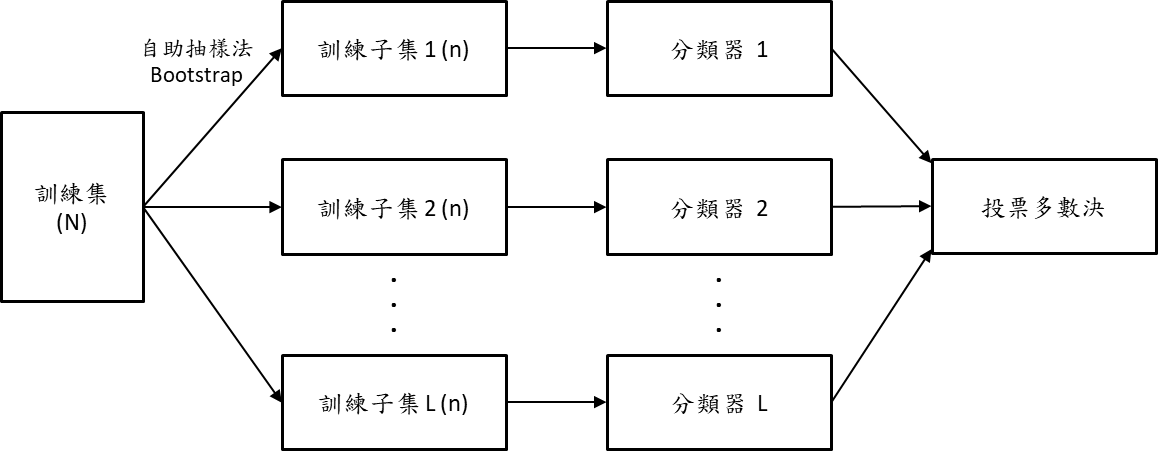
\includegraphics[width=1\textwidth]{figures/Image_Bagging.png}
      \caption[裝袋算法方式建樹示意圖]{裝袋算法方式建樹示意圖}
      \label{fig:Bagging}
    \end{center}
\end{figure}

\begin{figure}[!htb]
    \begin{center}
      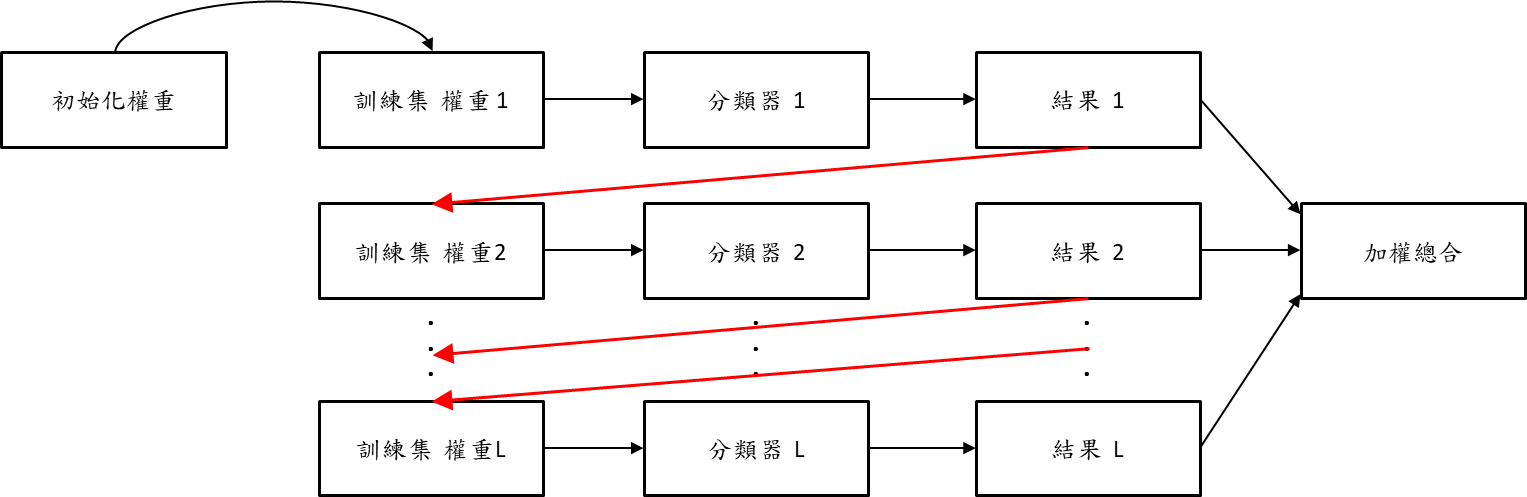
\includegraphics[width=1\textwidth]{figures/Image_Boosting.png}
      \caption[提升方法方式建樹示意圖]{提升方法方式建樹示意圖}
      \label{fig:Boosting}
    \end{center}
\end{figure}

Chen與Guestrin~\cite{chen2016xgboost}實作出高效率的梯度提升 ( Gradient Boosting ),稱其為極限梯度提升,除了使用提升方法建樹外,還針對錯誤修正的步驟,引入梯度下降法 ( Gradient Descent ) 的概念,加速了學習模型的收斂速度,使其修正錯誤的能力更加精準,大幅減少訓練的時間成本。近年來透過極限梯度提升來訓練的研究越來越多,且其預測能力皆有不錯的表現~\cite{XGBoostTemporalData}~\cite{martinez2020machine}~\cite{semenov2016performance}~\cite{janusz2017helping},明顯優於裝袋算法建樹方式的其他學習模型。

從上述得知,選用樹狀結構之學習模型將有助於預測分類問題,且其中使用極限梯度提升之成效最佳。因此,為求本論文之預測新進玩家流失能夠達到預期,將採用決策樹、隨機森林與極限梯度提升來驗證樹狀結構之優勢以及極限梯度提升之最佳表現。

\section{資料不平衡處理及其評估方式}

在遊戲領域進行機器學習訓練時,往往會遭受到資料不平衡的影響;例如:於預測是否付費上,非付費玩家會遠多於付費玩家,導致付費玩家資料過少~\cite{sifa2015predicting}。於預測是否流失上,流失玩家會遠多於非流失玩家,導致非流失玩家資料過少~\cite{lee2016predicting},前述研究都採以針對資料集進行處理的方式解決資料不平衡,例如:SMOTE (Synthetic Minority Over-sampling Technique),於少數群添加模擬資料,使得少數群之樣本數與多數群相等~\cite{chawla2002smote}。而本論文不只預測玩家是否會流失,還需分析其原因,如在資料集中填入模擬資料,將會使得分析失準,無法得到有效的資訊,所以我們將採用在機器學習訓練時,放大少數群之樣本權重值,使得學習模型更加著重於少數群的資訊,如同提升方法建樹時,藉由權重值的不同,修正分類錯誤的資訊~\cite{freund1999short}。

在評估資料不平衡資料集時,如果單純計算學習模型之 Precision、Recall 或 F - Score~\cite{chinchor1993muc},將導致多數群之評估結果壓過少數群之評估結果,使得最終評估失真,無法有效驗證學習模型之成效。因此,在評估不平衡資料時,Sifa等人額外運用幾何平均數 ( Geometric Mean )~\cite{kubat1997learning}來評估學習模型之成效~\cite{sifa2015predicting}。藉由上述的概念,本論文將採用 Weighted F$_{\beta}$ - Score 來評估不平衡資料,使得少數群之評估不被多數群所壓過,使用樣本間的數量權重差來計算多數群與少數群的 F$_{\beta}$ - Score,希望能夠合理的評估學習模型間的表現。